\chapter{Polynomien kertolasku}

\subsection*{Polynomin kertominen monomilla}

Polynomilausekkeiden käsittely on välttämätön taito matematiikassa, ja siksi tähän lukuun kannattaa paneutua kunnolla.

Polynomeja voi kertoa keskenään tuttujen reaalilukujen laskusääntöjen avulla. Yksinkertaisin erikoistapaus on polynomin kertominen monomilla.

\begin{esimerkki}
\qquad \\
\begin{itemize}
    \item $2x(3x^2+5x+7) = x2\cdot 3x^2+2x\cdot 5x+2x\cdot 7=6x^3+10x^2+14x$
    \item $5x(3y^2+4y) = 15xy^2+20xy$
    \item $x(y+z) = xy+xz$
    \item $2x(x+y+z) = 2x^2+2xy+2xz$
\end{itemize}
\end{esimerkki}

\subsection*{Kahden binomin tulo}

Toinen yksinkertainen tapaus on kahden binomin tulo. Tällöin päädytään kertomaan polynomit ensin termeittäin ja sitten laskemaan kaikki yhteen.

\begin{esimerkki}
\qquad \\
\begin{itemize}
    \item $(x+y)(z+w) = xz+xw+yz+yw$
    \item $(ax+by)(x+y) = ax^2+axy+bxy+by^2 = ax^2+(a+b)xy+by^2$
    \item $(x-5)(x-7) = x^2-7x-5x+35 = x^2-12x+35$
    \item $(ax-1)(x+6) = ax^2+6ax-x-6 = ax^2+(6a-1)x-6$
\end{itemize}
\end{esimerkki}

\subsection*{Yleinen kertolasku}

Osittelulain nojalla kahden polynomin tulo saadaan laskemalla yhteen kaikki
termit, jotka saadaan kertomalla termi ensimmäisestä ja toinen termi toisesta
polynomista.

\newcommand{\pbezier}[4]{
	\pgfmathsetmacro{\PBxa}{#1}
	\pgfmathsetmacro{\PBxb}{#2}
	\pgfmathsetmacro{\PBya}{#3}
	\pgfmathsetmacro{\PByb}{#3+#4}
	\pgfmathsetmacro{\PBca}{0.8 * \PBxa + 0.2 * \PBxb}
	\pgfmathsetmacro{\PBcb}{0.2 * \PBxa + 0.8 * \PBxb}
	\draw[color=red] (\PBxa, \PBya) .. controls (\PBca, \PByb) and (\PBcb, \PByb) .. (\PBxb, \PBya);
}

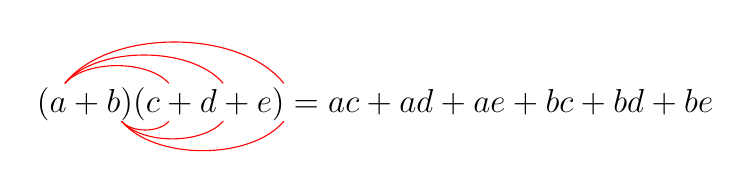
\begin{tikzpicture}
\draw node[right] {\large $(a+b)(c+d+e) = ac+ad+ae+bc+bd+be$};

\pgfmathsetmacro{\klAx}{0.48}
\pgfmathsetmacro{\klBx}{1.20}
\pgfmathsetmacro{\klCx}{1.8}
\pgfmathsetmacro{\klDx}{2.49}
\pgfmathsetmacro{\klEx}{3.26}
\pgfmathsetmacro{\klLo}{-0.22}
\pgfmathsetmacro{\klHi}{0.26}

\pbezier{\klAx}{\klCx}{\klHi}{0.3}
\pbezier{\klAx}{\klDx}{\klHi}{0.48}
\pbezier{\klAx}{\klEx}{\klHi}{0.7}

\pbezier{\klBx}{\klCx}{\klLo}{-0.15}
\pbezier{\klBx}{\klDx}{\klLo}{-0.3}
\pbezier{\klBx}{\klEx}{\klLo}{-0.5}
\end{tikzpicture}

Esimerkiksi polynomien $x-3$ ja $x^2-4x+3$ tulo voidaan laskea seuraavasti:
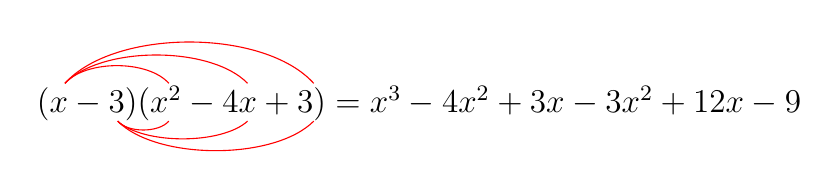
\begin{tikzpicture}
\draw node[right] {\large $(x-3)(x^2-4x+3) = x^3-4x^2+3x-3x^2+12x-9$};

\pgfmathsetmacro{\klAx}{0.48}
\pgfmathsetmacro{\klBx}{1.15}
\pgfmathsetmacro{\klCx}{1.8}
\pgfmathsetmacro{\klDx}{2.8}
\pgfmathsetmacro{\klEx}{3.64}
\pgfmathsetmacro{\klLo}{-0.22}
\pgfmathsetmacro{\klHi}{0.26}

\pbezier{\klAx}{\klCx}{\klHi}{0.3}
\pbezier{\klAx}{\klDx}{\klHi}{0.48}
\pbezier{\klAx}{\klEx}{\klHi}{0.7}

\pbezier{\klBx}{\klCx}{\klLo}{-0.15}
\pbezier{\klBx}{\klDx}{\klLo}{-0.3}
\pbezier{\klBx}{\klEx}{\klLo}{-0.5}
\end{tikzpicture}\newline
Vastaukseksi saadaan sievennyksen jälkeen $x^3-7x^2+15x-9$. (Tarkista itse!)

\begin{esimerkki}
\begin{align*}
&\hspace{0.5cm}(x^4-3x^3+3)(x^3-2x^2+1) \\
&= x^4 (x^3-2x^2+1) - 3x^3 (x^3-2x^2+1) + 3 (x^3-2x^2+1) \\
&= x^4\cdot x^3 + x^4\cdot (-2x^2)+x^4\cdot 1-3x^3\cdot x^3-3x^3(-2x^2)-3x^3\cdot1+3x^3+3(-2x^2)+3\cdot 1 \\
&= x^7-2x^6+x^4-3x^6+6x^5-3x^3+3x^3-6x^2+3 \\
&= x^7-5x^6+6x^5+x^4-6x^2+3
\end{align*}
\end{esimerkki}

\section{Muistikaavat}

Joitakin polynomien kertolaskuja tarvitaan niin usein, että niitä kutsutaan \termi[muistikaavoiksi]{muistikaavat}.

\laatikko{
    \textbf{Muistikaavat}
    \begin{itemize}
        \item $(a+b)^2 = a^2+2ab+b^2$
        \item $(a-b)^2 = a^2-2ab+b^2$
        \item $(a+b)(a-b) = a^2-b^2$
    \end{itemize}
}

Nämä kaavat voidaan todistaa helposti laskemalla.

\subsubsection*{Summan neliö}

\begin{align*}
(a+b)^2 &= (a+b)(a+b) &\emph{neliön määritelmä} \\
&= a(a+b)+b(a+b) &\emph{osittelulaki} \\
&= a^2+ab+ba+b^2 &\emph{osittelulaki} \\
&= a^2+ab+ab+b^2 &\emph{vaihdannaisuus ($ba=ab$)} \\
&= a^2+2ab+b^2
\end{align*}

\subsubsection*{Erotuksen neliö}

\begin{align*}
(a-b)^2 &= (a-b)(a-b) &\emph{neliön määritelmä} \\
&= a(a-b)-b(a-b) &\emph{osittelulaki} \\
&= a^2-ab-ba+b^2 &\emph{osittelulaki} \\
&= a^2-ab-ab+b^2 &\emph{vaihdannaisuus ($ba=ab$)} \\
&= a^2-2ab+b^2
\end{align*}

Edellä todistettuja kahta tapausta kutsutaan yhdessä nimellä binomin neliö. Toisinaan ne kirjoitetaan yhtenä yhtälönä muodossa $(a \pm b)^2=a^2 \pm 2ab+b^2$. Kaavoissa useasti esiintyviä $\pm$-merkkejä luetaan siten, että ylemmät ja alemmat täsmäävät keskenään. Ylempien merkkien (kaikki $+$:ia) valinta vastaa siis summan neliötä ja alempien merkkien (kaikki $-$:ia) valinta erotuksen neliötä.

\subsubsection*{Summan ja erotuksen tulo}

\begin{align*}
(a+b)(a-b) &= a(a-b)+b(a-b) &\emph{osittelulaki} \\
&= a^2-ab+ba-b^2 &\emph{osittelulaki} \\
&= a^2-ab+ab-b^2 &\emph{vaihdannaisuus ($ba=ab$)} \\
&= a^2-b^2
\end{align*}

\begin{esimerkki}
Kerro auki sulut lausekkeessa $(3x+2y)^2$. \\
Käytetään muistikaavaa $(a+b)^2 = a^2+2ab+b^2$. Nyt $a = 3x$ ja $b = 2y$.
Saadaan
        \[ (3x+2y)^2 = (3x)^2+2\cdot 3x\cdot 2y+(2y)^2 = 9x^2+12xy+4y^2. \]
\end{esimerkki}

\begin{esimerkki}
Laske päässä a) $995^2$ b) $104 \cdot 96$. \\
Käytetään ovelasti muistikaavoja $(a-b)^2 = a^2-2ab+b^2$ ja $(a+b)(a-b) = a^2-b^2$.
\begin{enumerate}[a)]
\item $995^2 = (1000-5)^2 = 1000^2-2\cdot 1000\cdot 5+5^2 = 1000000-10000+25 = 990025 $
\item $104\cdot 96 = (100+4)(100-4) = 100^2 - 4^2 = 10000 - 16 = 9984$.
\end{enumerate}
\end{esimerkki}

\section{Tekijöihinjako}

Pitkän matematiikan 1. kurssilla on käsitelty lukujen jakamista tekijöihin.
Esimerkiksi luvun $12$ \termi[tekijät]{tekijä} ovat luvut $1$, $2$, $3$, $4$, $6$ ja $12$. Nämä ovat sellaisia
lukuja, joista saadaan luku $12$ kertomalla ne jollain kokonaisluvulla, tai toisin sanottuna luku $12$ voidaan jakaa
millä tahansa näistä luvuista ilman jakojäännöstä.
%Sanotaan myös, että luvun $12$ \termi[alkutekijät]{alkutekijä} ovat $2$ ja $3$, koska luku $12$ voidaan
%ilmaista niiden tulona ($2\cdot 2\cdot 3 = 2^2\cdot 3 = 12$), mutta näitä tekijöitä ei
%voi enää jakaa pienempiin osatekijöihin. Kokonaisluvun tekijät ovat kokonaislukuja ja alkutekijät alkulukuja.

Polynomeja voidaan jakaa vastaavalla tavalla tekijöihin. Polynomien tapauksessa tekijöihinjako tarkoittaa
polynomin esittämistä saman- tai pienempiasteisten polynomien tulona. Aste on aina pienempi, ellei kyse ole pelkästä
vakiokertoimen ottamisesta yhteiseksi tekijäksi.

\begin{esimerkki}
\qquad \\
\begin{itemize}
    \item $x^2-1 = (x+1)(x-1)$
    \item $x^3+x = x(x^2+1)$
    \item $3x^2+6x = 3x(x+2)$
    \item $4x^2+24x+32 = 4(x+2)(x+4)$
\end{itemize}
\end{esimerkki}

On suositeltavaa tarkistaa itse, että yllä esitetyt tekijöihinjaot todella toimivat. Polynomien tekijöihinjaon toimivuus
on helppoa tarkistaa -- täytyy vain laskea väitettyjen tekijöiden tulo ja katsoa, onko se alkuperäinen polynomi. Vaikka
tarkistus onkin helppoa, tässä vaiheessa ei luultavasti vielä ole selvää, miten tekijöihinjaon voisi saada selville
-- paitsi toisinaan arvaamalla, mutta tähän kysymykseen vastataan myöhemmin tällä kurssilla.

Polynomien tekijöihinjako ei ole yksiselitteinen, mutta monesti hyödyllisintä on jakaa polynomi tekijöihin samoin kuin
esimerkkitapauksissa eli niin, että ensimmäisenä on vakiotermi ja kaikissa muissa tekijäpolynomeissa korkeimman asteen
termin kerroin on 1.

Esimerkki selkeyttänee asiaa. Polynomi $6x^2+30x+36$ voidaan jakaa tekijöihin vaikkapa seuraavilla tavoilla:

\begin{esimerkki}
\qquad \\
\begin{itemize}
    \item $6(x+2)(x+3)$
    \item $3(2x+4)(x+3)$
    \item $3(x+2)(2x+6)$
    \item $2(3x+6)(x+2)$
    \item $(6x+12)(x+3)$
    \item $(\frac12 x+1)(12x+36)$
\end{itemize}
\end{esimerkki}

Kaikki nämä tavat ovat ''oikein,'' mutta lähes aina ensimmäinen muoto $6(x+2)(x+3)$ on kätevin.

Toisinaan polynomeille voi löytää tekijöitä soveltamalla joitakin seuraavista keinoista:

\begin{itemize}
\item Otetaan korkeimman asteen termin kerroin yhteiseksi tekijäksi: \\
$5x^4+3x^2+x-9 = 5(x^4+\frac{3}{5} x^2+\frac{1}{5} x-\frac{9}{5})$
\item Otetaan $x$ tai sen potenssi yhteiseksi tekijäksi, jos mahdollista: \\
$x^5+x^3+3x = x(x^4+x^2+3)$
$x^7+x^6+5x^4+2x^2 = x^2(x^5+x^4+5x^2+2)$
\item Sovelletaan muistikaavaa käänteisesti \\
$x^2-5=x^2-\sqrt{5}^2=(x+\sqrt{5})(x-\sqrt{5})$ \\
$x^2+8x+16=x^2+2\cdot 4x+4^2=(x+4)^2$ \\
$x^2+x+\frac14=x^2+2\cdot \frac12 x+(\frac12)^2=(x+\frac12)^2$
\end{itemize}

\begin{esimerkki}
Jaetaan tekijöihin polynomi $10x^3-20x^2$.

\begin{align*}
& 10x^3-20x^2 \\
=& 10(x^3-2x^2) \ \ \ \ &\emph{otetaan $10$ yhteiseksi tekijäksi} \\
=& 10x^2(x-2) &\emph{otetaan $x^2$ yhteiseksi tekijäksi} \\
\end{align*}
\end{esimerkki}

\begin{esimerkki}
Jaetaan tekijöihin polynomi $5x^3-20x^2+20x$.

\begin{align*}
& 5x^3-20x^2+20x \\
=& 5(x^3-4x^2+4x) \ \ \ \ &\emph{otetaan $5$ yhteiseksi tekijäksi} \\
=& 5x(x^2-4x+4) &\emph{otetaan $x$ yhteiseksi tekijäksi} \\
=& 5x(x^2-2\cdot 2x+2^2) \\
=& 5x(x-2)^2 &\emph{sovelletaan muistikaavaa} \\
\end{align*}
\end{esimerkki}

Kaikkien polynomien tekijöihinjako ei kuitenkaan näillä menetelmillä onnistu. Myöhemmin tässä kirjassa opitaan,
miten polynomin voi jakaa tekijöihin nollakohtiensa avulla.

\Harjoitustehtavat

\subsubsection*{Opi perusteet}

\begin{tehtava}
    Sievennä.
    \begin{enumerate}[a)]
        \item $2(x+3)$
        \item $x(x - 2)$
        \item $3x(1-2x)$
        \item $x^2(x + 5)$
    \end{enumerate}
    \begin{vastaus}
        \begin{enumerate}[a)]
            \item $2x+6$
            \item $x^2 - 2x$
            \item $3x-6x^2$
            \item $x^3 + 5x$
        \end{enumerate}
    \end{vastaus}
\end{tehtava}

\begin{tehtava}
    Sievennä.
    \begin{enumerate}[a)]
        \item $3(x+2y-4)$
        \item $(x+2)(x + 3)$
        \item $(3-x)(2x-1)$
\end{enumerate}
    \begin{vastaus}
        \begin{enumerate}[a)]
            \item $3x+6y-12$
            \item $x^2 +5x+6$
            \item $-2x^2+7x-3$
        \end{enumerate}
    \end{vastaus}
\end{tehtava}

\begin{tehtava}
    Esitä tulona ottamalla yhteinen tekijä.
    \begin{enumerate}[a)]
        \item $2x+6$
        \item $x^2 -4x$
        \item $3x^2 - 6x$
    \end{enumerate}
    \begin{vastaus}
        \begin{enumerate}[a)]
        \item $2(x+3)$
        \item $x(x-4)$
        \item $3x(x-2)$
        \end{enumerate}
    \end{vastaus}
\end{tehtava}

\begin{tehtava}
    Kerro sulut auki muistikaavan avulla.
    \begin{enumerate}[a)]
        \item $(x+y)^2$
        \item $(x-y)^2$
        \item $(x+y)(x-y)$
        \item $(x+3)^2$
        \item $(y-5)^2$
        \item $(x-4)(x+4)$
        \item $(2x+1)^2$
    \end{enumerate}
    \begin{vastaus}
        \begin{enumerate}[a)]
        \item $x^2 +2xy+y^2$
        \item $x^2 -2xy +y^2$
        \item $x^2-y^2$
        \item $x^2 +6x+9$
        \item $y^2 - 10y+25$
        \item $x^2 -16$
        \item $4x^2 +4x +1$
        \end{enumerate}
    \end{vastaus}
\end{tehtava}



\subsubsection*{Hallitse kokonaisuutta}

\begin{tehtava}
    Sievennä.
    \begin{enumerate}[a)]
        \item $x(x^2 + 1)$
        \item $(x - 5)\cdot 3x$
        \item $(-2x)(4x - 1)\cdot 3$
        \item $2x(x + y)$
        \item $(3x^5 + 7)y$
        \item $(-x^3)(10x - 2)$
        \item $5(-2x + 1)(-9x) $
        \item $2x(x-3)+1$
    \end{enumerate}
    \begin{vastaus}
        \begin{enumerate}[a)]
            \item $x^3 + x$
            \item $3x^2 - 15x$
            \item $-24x^2 + 6x$
            \item $2x^2 + xy$
            \item $3x^5y + 7y$
            \item $-10x^4 + 2x^3$
            \item $90x^2 - 45x$
            \item $2x^2-6x+1$
        \end{enumerate}
    \end{vastaus}
\end{tehtava}

\begin{tehtava}
    Sievennä muistikaavojen avulla.
    \begin{enumerate}[a)]
        \item $(x+2)^2$
        \item $(x-3)^2$
        \item $(x-1)(x+1)$
        \item $(5-x)^2$
        \item $(2x + 8)^2$
        \item $(7x + 4)^2$
        \item $(9 - 7x)(9 + 7x)$
        \item $(8x - 8)(8x + 8)$
    \end{enumerate}
    \begin{vastaus}
        \begin{enumerate}[a)]
            \item $x^2 + 4x + 4$
            \item $x^2 - 6x + 9$
            \item $x^2 - 1$
            \item $x^2 - 10x + 25$
            \item $4x^2 + 32x + 64$
            \item $49x^2 + 56x + 16$
            \item $-49x^2 + 81$
            \item $64x^2 - 64$
        \end{enumerate}
    \end{vastaus}
\end{tehtava}

\begin{tehtava}
    Sievennä.
    \begin{enumerate}[a)]
        \item $(x+1)(x+3)$
        \item $(x+2)(x-1)$
        \item $(2x+5)(x+7)$
        \item $(x-1)(x+4)x$
    \end{enumerate}
    \begin{vastaus}
        \begin{enumerate}[a)]
            \item $x^2 + 4x + 3$
            \item $x^2 + x - 2$
            \item $2x^2 + 19x + 35$
            \item $x^3 + 3x^2 - 4x$
        \end{enumerate}
    \end{vastaus}
\end{tehtava}

\begin{tehtava}
    Sievennä.
    \begin{enumerate}[a)]
        \item $(t+v)^2+(t-v)^2$
        \item $(t+v)^2-(t-v)^2$
    \end{enumerate}
    \begin{vastaus}
        \begin{enumerate}[a)]
            \item $(t+v)^2+(t-v)^2 = t^2+2tv+v^2+t^2-2tv+v^2 = 2t^2+2v^2$
            \item $(t+v)^2-(t-v)^2 = t^2+2tv+v^2-t^2+2tv-v^2 = 4tv$
        \end{enumerate}
    \end{vastaus}
\end{tehtava}

\begin{tehtava}
	Laske 
	\begin{enumerate}[a)]
		\item $(x-3)(2x^3-3x+4)$
		\item $(x^2+1)(x^3-2x-4)$
		\item $(x-1)(x^4+x^3+x^2+x+1)$
		\item $(\frac x5-\frac23)(x^2+x+1)$
	\end{enumerate}
	\begin{vastaus}
		\begin{enumerate}[a)]
			\item $2x^4-6x^3-3x^2+13x-12$
			\item $x^5-x^3-4x^2-2x-4$
			\item $x^5-1$
			\item $\frac15x^3-\frac{7}{15}x^2-\frac{7}{15}x-\frac23$
		\end{enumerate}
	\end{vastaus}
\end{tehtava}

\begin{tehtava}
    Johda ''muistikaavat'' potenssien
    \begin{enumerate}[a)]
            \item $(a+b)^3$
            \item $(a+b)^4$
            \item $(a-b)^3$
        \end{enumerate}
        aukikertomiseksi.
    \begin{vastaus}
        \begin{enumerate}[a)]
            \item $(a+b)^3 = a^3 + 3a^2b + 3ab^2 + b^3$
            \item $(a+b)^4 = a^4 + 4a^3b + 6a^2b^2 + 4ab^3 + b^4$
            \item $(a-b)^3 = a^3 - 3a^2b + 3ab^2 - b^3$
        \end{enumerate}
    \end{vastaus}
\end{tehtava}

\begin{tehtava} %Vaikea!
    Kahden luvun keskiarvo on $7$. Kuinka suuri niiden tulo voi korkeintaan olla?
    \begin{vastaus}
        $49$. Perustelu muistikaavoilla: $(7+a)(7-a)=7^2-a^2 = 49-a^2 \geq 49$
    \end{vastaus}
\end{tehtava}

\subsubsection*{Sekalaisia, lajittele}

\begin{tehtava}
    Sievennä lauseke $(x^2+1)(x^3-2x)$. Mikä on polynomin aste?
    \begin{vastaus}
        Lauseke sievenee muotoon $x^5-x^3-2x$. Polynomin aste on $5$.
    \end{vastaus}
\end{tehtava}

\begin{tehtava}
    Määritä sulkuja avaamatta lausekkeen $(x^2+1)(x^3-2x)$
    \begin{enumerate}[a)]
        \item aste
        \item vakiotermi.
    \end{enumerate}
    \begin{vastaus}
        \begin{enumerate}[a)]
            \item Polynomin aste on kunkin tekijän korkeimpien asteiden summa, tässä siis $2+3=5$.
            \item Polynomin vakiotermi on kunkin tekijän vakiotermien tulo, tässä siis $1\cdot 0=0$.
        \end{enumerate}
    \end{vastaus}
\end{tehtava}


\begin{tehtava}
    Sievennä. (Ohje: käytä summakaavoja.)
    \begin{enumerate}[a)]
        \item $63^2+37^2$
        \item $101^2+99^2$
    \end{enumerate}
    \begin{vastaus}
        \begin{enumerate}[a)]
            \item $63^2+37^2 = (50+13)^2+(50-13)^2 = 2\cdot 50^2 + 2\cdot 13^2 = 2\cdot 2500 +2\cdot 169 = 5000 + 338 = 5338$
            \item $101^2+99^2 = (100+1)^2+(100-1)^2 = 2\cdot 100^2 + 2\cdot 1^2 = 2\cdot 10000 + 2\cdot 1 = 20000 + 2 = 20002$
        \end{enumerate}
    \end{vastaus}
\end{tehtava}

\begin{tehtava}
    Sievennä.
    \begin{enumerate}[a)]
        \item $35^2-25^2$
        \item $170^2-50^2$
    \end{enumerate}
    \begin{vastaus}
        \begin{enumerate}[a)]
            \item $35^2-25^2 = (30+5)^2-(30-5)^2 = 4\cdot 30\cdot 5 = 600$
            \item $170^2-30^2 = (100+70)^2+(100-70)^2 = 4\cdot 100\cdot 70 = 28000$
        \end{enumerate}
    \end{vastaus}
\end{tehtava}

\begin{tehtava}
    Olkoon $P(x)=-x^4+2x$ reaalifunktio. Sievennä lausekkeet.
    \begin{enumerate}[a)]
		\item $P(\sqrt{2})$
        \item $P(x)^2$
        \item $P(-x)$
        \item $P(2t)$
    \end{enumerate}
    \begin{vastaus}
        \begin{enumerate}[a)]
            \item $-4 + 2\sqrt{2}$
            \item $x^8 - 4x^5 + 4x^2$
            \item $-x^4-2x$
            \item $-16t^4+4t$
        \end{enumerate}
    \end{vastaus}
\end{tehtava}

\begin{tehtava}
    Olkoot $P(x)=x^2$ ja $Q(x)=x+1$ reaalifunktioita. Sievennä lausekkeet.
    \begin{enumerate}[a)]
        \item $P(x+1)$
        \item $Q(x-1)$
        \item $P(Q(x))$
        \item $Q(P(x))$
    \end{enumerate}
    \begin{vastaus}
        \begin{enumerate}[a)]
            \item $P(x+1) = (x+1)^2 = x^2+2x+1$
            \item $Q(x-1) = (x-1)+1 = x$
            \item $P(Q(x)) = P(x+1) = (x+1)^2 = x^2+2x+1$
            \item $Q(P(x)) = Q(x^2) = x^2+1$
        \end{enumerate}
    \end{vastaus}
\end{tehtava}
